% 逻辑主线: 描述AI发展的现状及核心挑战,分析造成这些挑战的具体原因,并探讨潜在的解决方向。

% 第3章:阻碍AI发展的主要挑战
% \section{Challenges to AI Development}
\section{Scaling at Risk: Challenges of Data and Computing Power}

% 3.1 Scaling Law正在失效
% \subsection{The Breakdown of Scaling Laws}
% - 当前Scaling Law是否仍然适用?(模型规模扩张带来的性能提升是否逐渐滞后?)
% - 为什么Scaling Law正在失效?(训练数据和算力扩展的矛盾,数据规模增长超出模型规模等具体原因)
% - 如果Scaling Law失效,将对AI模型发展带来什么影响?(技术提升进入瓶颈,无法通过简单扩张规模解决问题)

% 3.2 数据用尽:公共数据的天花板
% \subsection{Data Exhaustion: The Ceiling of Public Data}
\subsection{The Ceiling of Public Data}
\label{subsec:data_exhaustion}
% - 现有公共数据为何不足以支撑AI模型进一步扩展?(数据质量和数量饱和问题)
% - AIGC(生成式AI)时代对数据有什么影响?(生成式内容污染公共数据源,合成数据质量差而无法替代真实数据)
% - 数据枯竭问题将对大规模模型训练带来什么危机?(数据基础的缺陷导致模型扩展难以为继)

% \begin{figure}
%     \centering
% 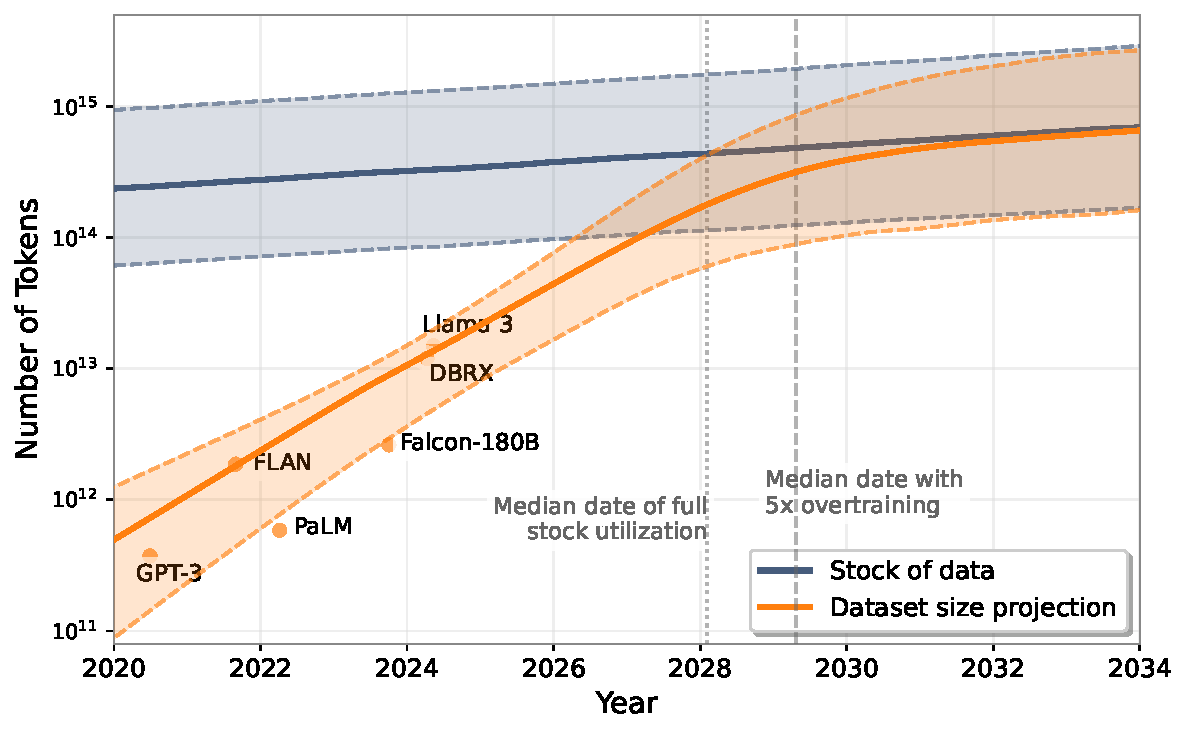
\includegraphics[width=\linewidth]{figs/projections.pdf}
%     \caption{Comparison between the projected growth of available public training data (\textcolor[RGB]{70,92,124}{blue}) and model dataset size requirements (\textcolor[RGB]{255, 127, 14}{orange}) from 2020 to 2034. The available stock of public training data will be fully utilized by around 2028.}
%     \label{fig:proj}
% \end{figure}

% 数据的需求很高
% \textbf{The Imminence of Data Exhaustion.} 
% With the rapid development of LLMs, the demand for data is growing exponentially. According to neural scaling laws, the improvement in model performance relies on the increase in the scale of training data \cite{hoffmann2022training}. 
% % Taking GPT-3 as an example, its training dataset size has reached hundreds of billions of tokens, encompassing diverse data types such as books, web pages, and code \cite{brown2020language}. 
% Taking GPT-3 as an example, its training dataset size has reached 300 billion tokens, encompassing diverse data types such as books, web pages, and code \cite{brown2020language}. 
% Research indicates that the size of training datasets is growing at a rate of approximately 0.38 orders of magnitude (about 2.4 times) per year \cite{villalobos2022trends}. 
% If this trend continues, models will require significantly more data in the coming years to sustain performance improvements.




% % 数据的供给赶不上需求
% However, despite the vast scale of publicly available human-generated text data on the internet, its total quantity is finite. 
% Estimates suggest that the current stock of publicly available human-generated text data is around 4e14 tokens (approximately 400 trillion tokens) \cite{villalobos2022trends}. 
% As shown in Figure~\ref{fig:proj}, if the current trends in LLM development persist, models are expected to exhaust the entire stock of publicly available human-generated text data by around 2028 \cite{villalobos2024will}. 
% If models are overtrained, this timeline could be accelerated to as early as 2026 \cite{villalobos2024will}. 
% Overtraining refers to the practice of using more data than what is compute-optimal during model training. While this can improve inference efficiency, it accelerates the consumption of data.
% Data exhaustion will lead to a stagnation in model performance improvements unless new data sources are found or data efficiency is enhanced.
% % The expansion of computational resources is also constrained by factors such as energy efficiency and chip production capacity \cite{ho2023limits}. 
% Therefore, the finite nature of publicly available human-generated text data is expected to become a major bottleneck for LLM scaling within the next decade. Despite the current large scale of public data, the risk of data exhaustion is rapidly approaching as data demand continues to grow \cite{sevilla2022compute}.



% % \textbf{Potential and Challenges of Synthetic Data.}
% Faced with the threat of data exhaustion, researchers have proposed various solutions, among which synthetic data generation is considered one of the most promising approaches. By using foundation models to generate data themselves, it is theoretically possible to infinitely expand the scale of training data. For example, OpenAI generates 100 billion words of text data daily, approaching the total volume of high-quality text in the Common Crawl dataset \cite{griffin2024chatgpt}. The advantages of synthetic data lie in its scalability and low cost, especially in specific domains such as mathematics, programming, and games, where synthetic data has already demonstrated significant effectiveness \cite{yang2023leandojo, liu2023tinygsm}.

% However, the use of synthetic data also faces numerous challenges. 
% First, model collapse is a serious issue. When models repeatedly train on their own generated data, they may gradually deviate from the original data distribution, leading to increasingly homogeneous and less diverse outputs \cite{shumailov2023curse}. 
% Research shows that iterative training on synthetic data can result in performance degradation and even negative returns \cite{singh2023beyond}. 
% Second, the quality of synthetic data is difficult to guarantee. While in certain domains (such as mathematical proofs), the effectiveness of synthetic data can be ensured through verification mechanisms, in complex tasks like natural language processing, the quality of synthetic data is often hard to evaluate \cite{alemohammad2023self}.
% Additionally, the diversity of synthetic data is a critical issue. To ensure that models can learn a broad range of knowledge, synthetic data needs to cover diverse linguistic styles, topics, and cultural contexts. However, existing synthetic data generation methods often struggle to produce sufficiently diverse data, limiting their application in general-purpose language models \cite{fan2023scaling}. Therefore, although synthetic data has shown promise in specific tasks, its widespread application in general language models requires further research and technological breakthroughs.



\paragraph{Public data for pretraining is exhausting.} The rapid advancement of large language models has created an insatiable appetite for training data. Neural scaling laws establish that model performance improves predictably with data quantity—a relationship that demands exponentially growing datasets \cite{hoffmann2022training}. A canonical example is GPT-3, trained on {300 billion tokens} spanning books, web content, and programming code \cite{brown2020language}. Current projections suggest dataset sizes grow at 0.38 orders of magnitude (2.4$\times$) annually \cite{villalobos2022trends}, implying models will require {three orders of magnitude more data} within a decade.

Despite the internet's vast textual resources, the total stock of high-quality human-generated text remains bounded. Recent estimates place this limit at approximately {$4\times 10^{14}$ tokens} \cite{villalobos2022trends}. \citet{villalobos2024will} argues that current consumption patterns suggest exhaustion of public text data by 2028, potentially accelerated to 2026 through excessive data reuse during training (a practice termed {overtraining}). 
% This creates a fundamental tension: while additional data currently drives progress, unrestrained consumption threatens future advancement.
Therefore, the finite nature of publicly available human-generated text data is expected to become a major bottleneck for LLM scaling within the next decade. Despite the current large scale of public data, the risk of data exhaustion is rapidly approaching as data demand continues to grow \cite{sevilla2022compute}.

% Synthetic data generation presents a paradoxical opportunity. 
\paragraph{Synthetic data has potential but faces challenges.}
Faced with the threat of data exhaustion, researchers have proposed various solutions, among which synthetic data generation is considered one of the most promising approaches. 
By leveraging LLMs to produce their own training data, researchers envision {self-sustaining data ecosystems}. Early successes in constrained domains like mathematics and code generation, where automated verification ensures quality, demonstrate potential \cite{liu2023tinygsm}.  Recent work \cite{chen2024diversity} demonstrated that diverse synthetic data enhances the performance of LLMs during both pre-training and fine-tuning.

% Industrial implementations already achieve remarkable scale—OpenAI reportedly generates {100 billion synthetic tokens daily}, rivaling major web-crawled corpora \cite{griffin2024chatgpt}.

The adoption of synthetic data faces three fundamental challenges. First, \textit{model collapse} occurs when models iteratively train on their own outputs, causing gradual divergence from original data distributions. This recursive process amplifies biases and reduces output diversity, ultimately degrading model performance across generations \cite{shumailov2023curse,dohmatob2024strong}. 
Second, \textit{synthetic data quality} remains inherently unverifiable in open-domain contexts. While formal domains like mathematics allow algorithmic validation, natural language lacks objective evaluation standards. The absence of ground-truth verification creates self-referential quality assessments, compromising reliability \cite{alemohammad2023self,wenger2024ai}.
Finally, synthetic data struggles to replicate human \textit{linguistic diversity}. Current methods disproportionately replicate dominant language patterns while underrepresenting cultural nuances and low-frequency expressions. This homogeneity limits their utility for training robust general-purpose models \cite{fan2023scaling}.

These persistent challenges underscore that synthetic data alone cannot sustainably address the looming data scarcity crisis, compelling the research community to seek complementary strategies that transcend conventional data acquisition paradigms.





% 3.3 算力垄断与成本高企
% \subsection{Computing Power Monopoly and High Costs}\label{subsec:compute_monopoly}
\subsection{The Monopoly of Computing Resources}\label{subsec:compute_monopoly}
\paragraph{A few AI giants dominate the computing power.}
The AI computing landscape is dominated by a few major tech giants like OpenAI, Google, Microsoft, and Meta, which control powerful hardware such as GPUs and TPUs. This monopolization creates a significant barrier for smaller AI startups and research institutions, who struggle to access such advanced resources. Additionally, these companies control proprietary AI models, datasets, and software frameworks that require immense computing power, further widening the gap between the giants and smaller players. As a result, high-performance computing resources remain increasingly inaccessible to anyone outside these dominant entities.

\begin{figure}
    \centering
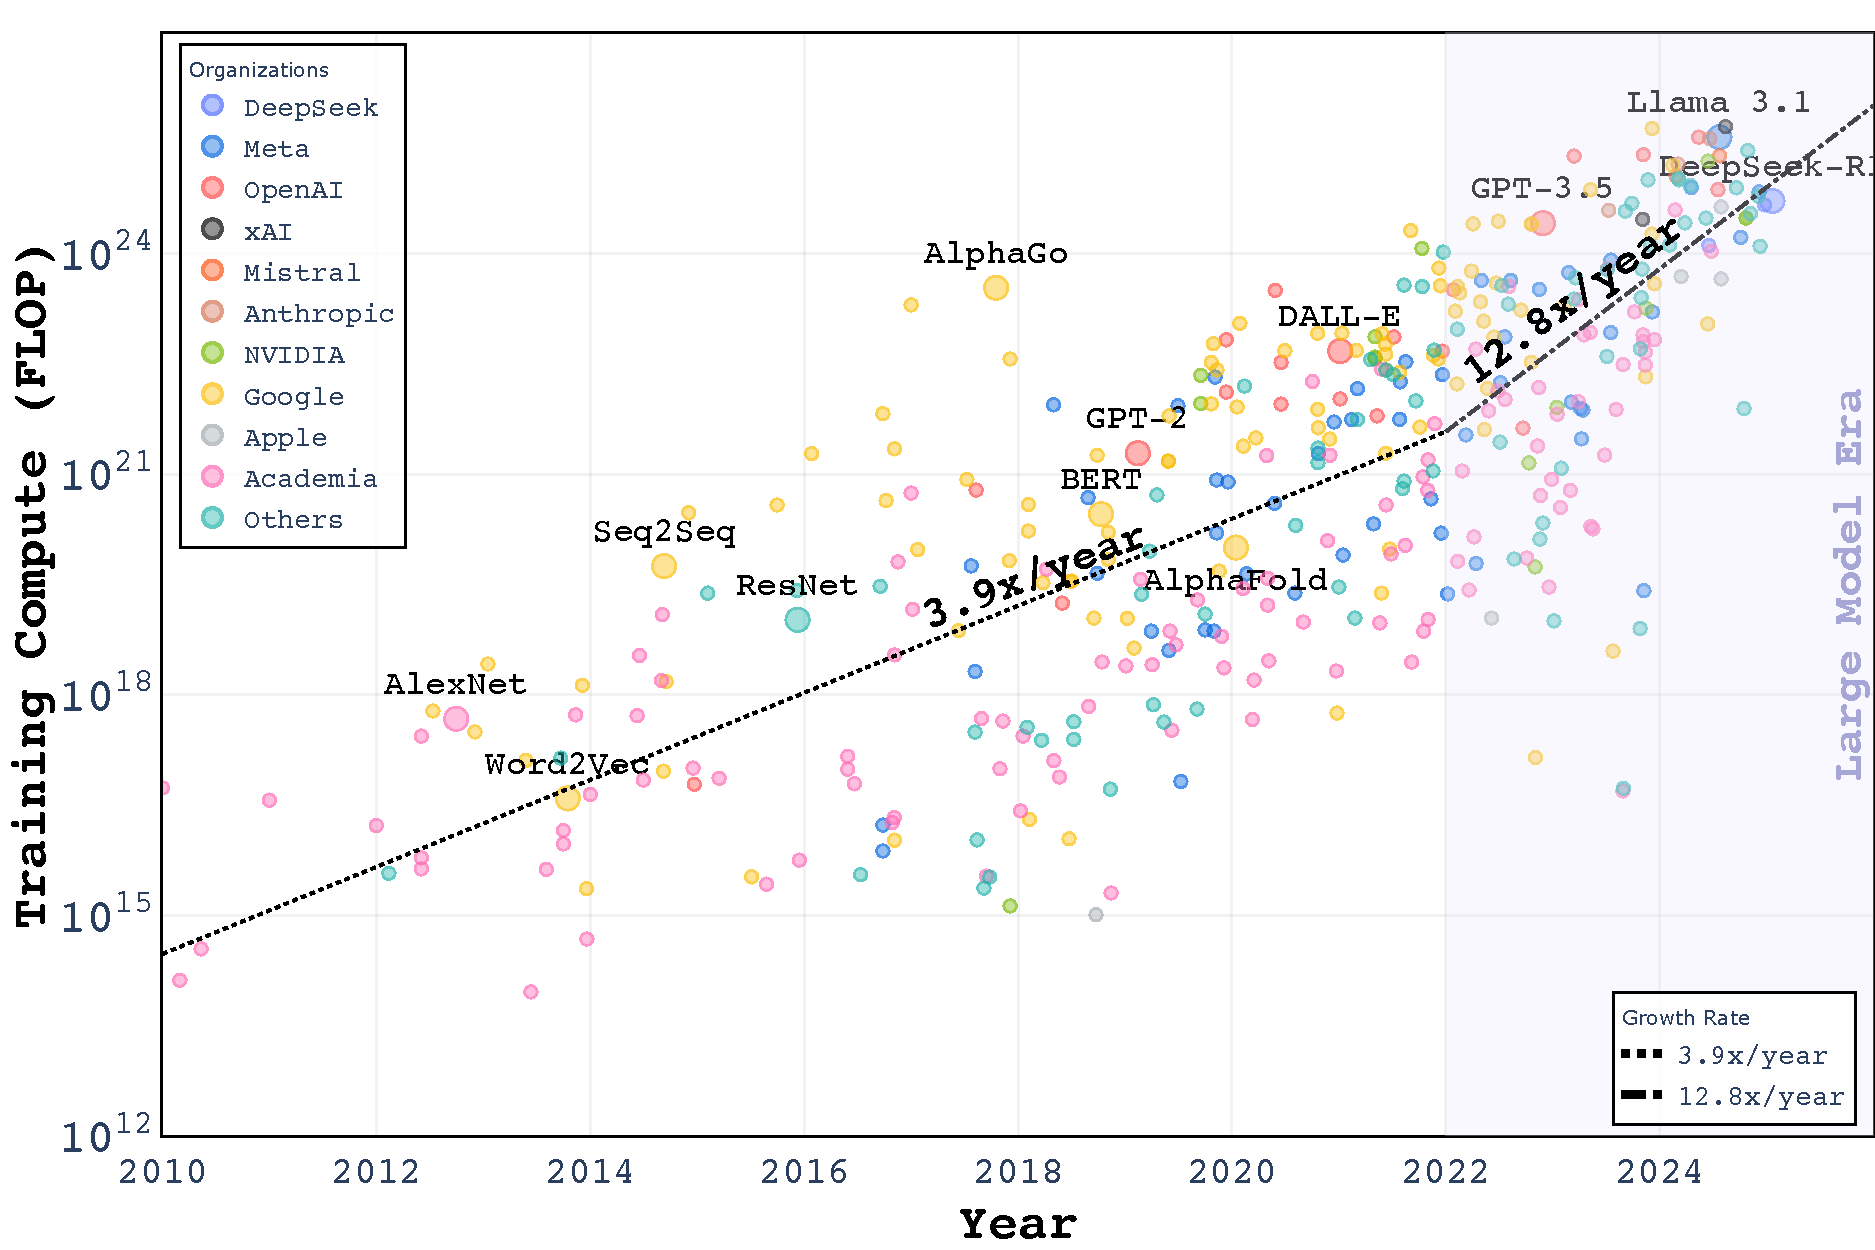
\includegraphics[width=\linewidth]{./figs/ai_compute_trend.pdf}
\vspace{-20pt}
    \caption{Trend of Computational Demand for Model Training. (Data source: Notable AI models~\cite{epoch2023trendsinmachinelearninghardware}).}
    \label{fig:model_comput_trend}
\end{figure}


\paragraph{Computational demand is growing exponentially.}
As large-scale AI models like GPT-4~\cite{openai2023gpt4}, Llama 3~\cite{meta2024llama3.1}, and DeepSeek-V3~\cite{liu2024deepseek} surpass the trillion-parameter scale, the global AI landscape faces severe computational efficiency challenges. As shown in Figure~\ref{fig:model_comput_trend}, since the deep learning revolution in 2010, AI training demands have grown at a super-exponential rate of 3.9$\times$ per year—an acceleration that intensified with the adoption of the transformer architecture as the industry standard \cite{vaswani2017attention}. With the advent of the era of large language models in 2022, the demand for computing power has surged even further, reaching an unprecedented growth rate of 13.4$\times$ per year. This marks a transformative shift in AI computation, where the need for computing power is expanding at an unprecedented pace, pushing the limits of existing hardware and infrastructure.

% Take Meta's Llama 3 as an example: its 405 billion parameters require a computing cluster of 24,000 NVIDIA H100 GPUs, consuming 30.8 million GPU hours—the equivalent of a single GPU running non-stop for 3,516 years. The hardware alone costs \$720 million while factoring in power, cooling, and operational expenses pushes total training costs beyond \$900 million. This surge in computational demand has created a triple-layered technical bottleneck. The first challenge lies in the \textbf{rapid expansion of model sizes}. The "New Moore's Law" projects a 40× increase in model parameters every 18 months, dramatically extending training cycles from weeks to months \cite{fan2023scaling}. The second challenge stems from the \textbf{escalating complexity of parallel computing architectures}. Ensuring training efficiency now requires exponentially more intricate hybrid strategies for data and model parallelism, demanding hundreds of engineer-months for optimization. Finally, the \textbf{hardware constraints} are increasingly prohibitive, with high-precision training presenting significant challenges in terms of memory bandwidth and interconnect requirements, pushing the limits of existing computing infrastructure.



\paragraph{Moore's Law is slowing down.}
Moore's Law, which has driven the growth in computing power for decades, is slowing down as we approach the physical limits of silicon-based chip technology~\cite{kressel2023end}. The difficulty in shrinking transistors has led to diminishing returns in computational performance. As a result, the AI industry is relying more on specialized hardware like GPUs, TPUs, and custom chips to meet growing demands. However, this shift has made high-performance hardware even more expensive and exclusive, further intensifying the gap between organizations with the resources to develop advanced AI models and those without.

\paragraph{Infrastructure capacity is a constraint.}
% The rapid growth in AI model size and computational demand has exposed significant capacity constraints in global computing infrastructure. Despite advances in specialized hardware, the resources required to train state-of-the-art models are outpacing existing data center capacities, leading to logistical challenges in scaling up production. Additionally, the immense energy consumption needed for these computations raises environmental concerns, contributing to a growing carbon footprint. Until more energy-efficient hardware and sustainable practices are developed, these cost and environmental issues will remain key challenges.
The rapid expansion of AI model scales and the surge in computational demand are facing dual constraints in global computing infrastructure. On one hand, bottlenecks in advanced semiconductor manufacturing severely limit the expansion rate of AI data centers. The foundry capacity for wafers at 5nm and below—such as those produced by TSMC—has already been fully booked by leading technology companies until 2026~\cite{benzinga2024tsmc}. Moreover, the construction of new wafer fabs involves long lead times and is further constrained by the global supply chain shortages of critical equipment, such as lithography machines.
On the other hand, the exponential increase in chip deployment within individual AI clusters is putting immense pressure on the already limited semiconductor manufacturing capacity, pushing the industry toward its production ceiling~\cite{scaleflux2024ai}.
These factors have significantly hindered the continuous expansion of computing power, making it increasingly difficult to scale AI infrastructure sustainably.

% - 当前算力资源的分布情况如何?(极少数AI巨头垄断了绝大部分算力资源)
% - 大规模算力需求是如何增加的?(从BERT到GPT-4算力曲线的指数级增长,模型扩展带来的成本上涨)
% - 摩尔定律放缓。
% - 产能

% % 3.4 解决方向概述
% \subsection{Overview of Potential Solutions}
% % - 针对上述挑战,有哪些方向可以探索?(例如,更高效的数据利用方式、更具普惠性的算力分布)
% % - 对于Scaling Law失效、数据枯竭和算力瓶颈,联邦学习和边缘设备是否有潜力成为解决方案?